% Options for packages loaded elsewhere
\PassOptionsToPackage{unicode}{hyperref}
\PassOptionsToPackage{hyphens}{url}
%
\documentclass[
  11pt,
]{article}
\usepackage{amsmath,amssymb}
\usepackage{lmodern}
\usepackage{iftex}
\ifPDFTeX
  \usepackage[T1]{fontenc}
  \usepackage[utf8]{inputenc}
  \usepackage{textcomp} % provide euro and other symbols
\else % if luatex or xetex
  \usepackage{unicode-math}
  \defaultfontfeatures{Scale=MatchLowercase}
  \defaultfontfeatures[\rmfamily]{Ligatures=TeX,Scale=1}
\fi
% Use upquote if available, for straight quotes in verbatim environments
\IfFileExists{upquote.sty}{\usepackage{upquote}}{}
\IfFileExists{microtype.sty}{% use microtype if available
  \usepackage[]{microtype}
  \UseMicrotypeSet[protrusion]{basicmath} % disable protrusion for tt fonts
}{}
\makeatletter
\@ifundefined{KOMAClassName}{% if non-KOMA class
  \IfFileExists{parskip.sty}{%
    \usepackage{parskip}
  }{% else
    \setlength{\parindent}{0pt}
    \setlength{\parskip}{6pt plus 2pt minus 1pt}}
}{% if KOMA class
  \KOMAoptions{parskip=half}}
\makeatother
\usepackage{xcolor}
\IfFileExists{xurl.sty}{\usepackage{xurl}}{} % add URL line breaks if available
\IfFileExists{bookmark.sty}{\usepackage{bookmark}}{\usepackage{hyperref}}
\hypersetup{
  pdftitle={SURVIVAL ANALYSIS - TCGA PRAD CANCER},
  pdfauthor={Kelvin Ofori-Minta; University of Texas at El Paso (UTEP)},
  hidelinks,
  pdfcreator={LaTeX via pandoc}}
\urlstyle{same} % disable monospaced font for URLs
\usepackage[margin=1in]{geometry}
\usepackage{color}
\usepackage{fancyvrb}
\newcommand{\VerbBar}{|}
\newcommand{\VERB}{\Verb[commandchars=\\\{\}]}
\DefineVerbatimEnvironment{Highlighting}{Verbatim}{commandchars=\\\{\}}
% Add ',fontsize=\small' for more characters per line
\usepackage{framed}
\definecolor{shadecolor}{RGB}{248,248,248}
\newenvironment{Shaded}{\begin{snugshade}}{\end{snugshade}}
\newcommand{\AlertTok}[1]{\textcolor[rgb]{0.94,0.16,0.16}{#1}}
\newcommand{\AnnotationTok}[1]{\textcolor[rgb]{0.56,0.35,0.01}{\textbf{\textit{#1}}}}
\newcommand{\AttributeTok}[1]{\textcolor[rgb]{0.77,0.63,0.00}{#1}}
\newcommand{\BaseNTok}[1]{\textcolor[rgb]{0.00,0.00,0.81}{#1}}
\newcommand{\BuiltInTok}[1]{#1}
\newcommand{\CharTok}[1]{\textcolor[rgb]{0.31,0.60,0.02}{#1}}
\newcommand{\CommentTok}[1]{\textcolor[rgb]{0.56,0.35,0.01}{\textit{#1}}}
\newcommand{\CommentVarTok}[1]{\textcolor[rgb]{0.56,0.35,0.01}{\textbf{\textit{#1}}}}
\newcommand{\ConstantTok}[1]{\textcolor[rgb]{0.00,0.00,0.00}{#1}}
\newcommand{\ControlFlowTok}[1]{\textcolor[rgb]{0.13,0.29,0.53}{\textbf{#1}}}
\newcommand{\DataTypeTok}[1]{\textcolor[rgb]{0.13,0.29,0.53}{#1}}
\newcommand{\DecValTok}[1]{\textcolor[rgb]{0.00,0.00,0.81}{#1}}
\newcommand{\DocumentationTok}[1]{\textcolor[rgb]{0.56,0.35,0.01}{\textbf{\textit{#1}}}}
\newcommand{\ErrorTok}[1]{\textcolor[rgb]{0.64,0.00,0.00}{\textbf{#1}}}
\newcommand{\ExtensionTok}[1]{#1}
\newcommand{\FloatTok}[1]{\textcolor[rgb]{0.00,0.00,0.81}{#1}}
\newcommand{\FunctionTok}[1]{\textcolor[rgb]{0.00,0.00,0.00}{#1}}
\newcommand{\ImportTok}[1]{#1}
\newcommand{\InformationTok}[1]{\textcolor[rgb]{0.56,0.35,0.01}{\textbf{\textit{#1}}}}
\newcommand{\KeywordTok}[1]{\textcolor[rgb]{0.13,0.29,0.53}{\textbf{#1}}}
\newcommand{\NormalTok}[1]{#1}
\newcommand{\OperatorTok}[1]{\textcolor[rgb]{0.81,0.36,0.00}{\textbf{#1}}}
\newcommand{\OtherTok}[1]{\textcolor[rgb]{0.56,0.35,0.01}{#1}}
\newcommand{\PreprocessorTok}[1]{\textcolor[rgb]{0.56,0.35,0.01}{\textit{#1}}}
\newcommand{\RegionMarkerTok}[1]{#1}
\newcommand{\SpecialCharTok}[1]{\textcolor[rgb]{0.00,0.00,0.00}{#1}}
\newcommand{\SpecialStringTok}[1]{\textcolor[rgb]{0.31,0.60,0.02}{#1}}
\newcommand{\StringTok}[1]{\textcolor[rgb]{0.31,0.60,0.02}{#1}}
\newcommand{\VariableTok}[1]{\textcolor[rgb]{0.00,0.00,0.00}{#1}}
\newcommand{\VerbatimStringTok}[1]{\textcolor[rgb]{0.31,0.60,0.02}{#1}}
\newcommand{\WarningTok}[1]{\textcolor[rgb]{0.56,0.35,0.01}{\textbf{\textit{#1}}}}
\usepackage{graphicx}
\makeatletter
\def\maxwidth{\ifdim\Gin@nat@width>\linewidth\linewidth\else\Gin@nat@width\fi}
\def\maxheight{\ifdim\Gin@nat@height>\textheight\textheight\else\Gin@nat@height\fi}
\makeatother
% Scale images if necessary, so that they will not overflow the page
% margins by default, and it is still possible to overwrite the defaults
% using explicit options in \includegraphics[width, height, ...]{}
\setkeys{Gin}{width=\maxwidth,height=\maxheight,keepaspectratio}
% Set default figure placement to htbp
\makeatletter
\def\fps@figure{htbp}
\makeatother
\setlength{\emergencystretch}{3em} % prevent overfull lines
\providecommand{\tightlist}{%
  \setlength{\itemsep}{0pt}\setlength{\parskip}{0pt}}
\setcounter{secnumdepth}{5}
\usepackage{amsmath}
\usepackage{amssymb, bm}
\usepackage{amsfonts}
\usepackage{amsthm}
\usepackage{fancyhdr}
\pagestyle{fancy}
\fancyhf{}
\rhead{Collaborative Research}
\lhead{TCGA - Clinical Data}
\cfoot{\thepage}
\usepackage{algorithm}
\usepackage[noend]{algpseudocode}
\usepackage{booktabs}
\usepackage{longtable}
\usepackage{array}
\usepackage{multirow}
\usepackage{wrapfig}
\usepackage{float}
\usepackage{colortbl}
\usepackage{pdflscape}
\usepackage{tabu}
\usepackage{threeparttable}
\usepackage{threeparttablex}
\usepackage[normalem]{ulem}
\usepackage{makecell}
\usepackage{xcolor}
\ifLuaTeX
  \usepackage{selnolig}  % disable illegal ligatures
\fi

\title{SURVIVAL ANALYSIS - TCGA PRAD CANCER}
\author{Kelvin Ofori-Minta \and University of Texas at El Paso (UTEP)}
\date{June 20, 2022}

\begin{document}
\maketitle

{
\setcounter{tocdepth}{4}
\tableofcontents
}
\newpage
\section{Loading and Cleaning Data}

\begin{Shaded}
\begin{Highlighting}[]
\NormalTok{data }\OtherTok{\textless{}{-}} \FunctionTok{read.csv}\NormalTok{(}\StringTok{"neoplasm.status\_withtumor.csv"}\NormalTok{, }\AttributeTok{header =}\NormalTok{ T, }\AttributeTok{stringsAsFactors =}\NormalTok{ F,}
              \AttributeTok{na.strings =} \StringTok{"NA"}\NormalTok{)}
\CommentTok{\#selecting columns of interest}
\CommentTok{\#data\textless{}{-}s[, c(4,7,8,12,13,19,20,21,23,27:32,44:47,50,53:55,58,62,40:42)]}
\CommentTok{\# write.csv(data,"C://Users//Kelvin//Desktop//Spring 2022//research with Dr. Leung//survival//selected\_columns.csv")}
\end{Highlighting}
\end{Shaded}

\subsection{Inspecting dataframe for missing values}

\begin{Shaded}
\begin{Highlighting}[]
\FunctionTok{require}\NormalTok{(inspectdf)}
\FunctionTok{show\_plot}\NormalTok{(}\FunctionTok{inspect\_na}\NormalTok{(data))}
\end{Highlighting}
\end{Shaded}

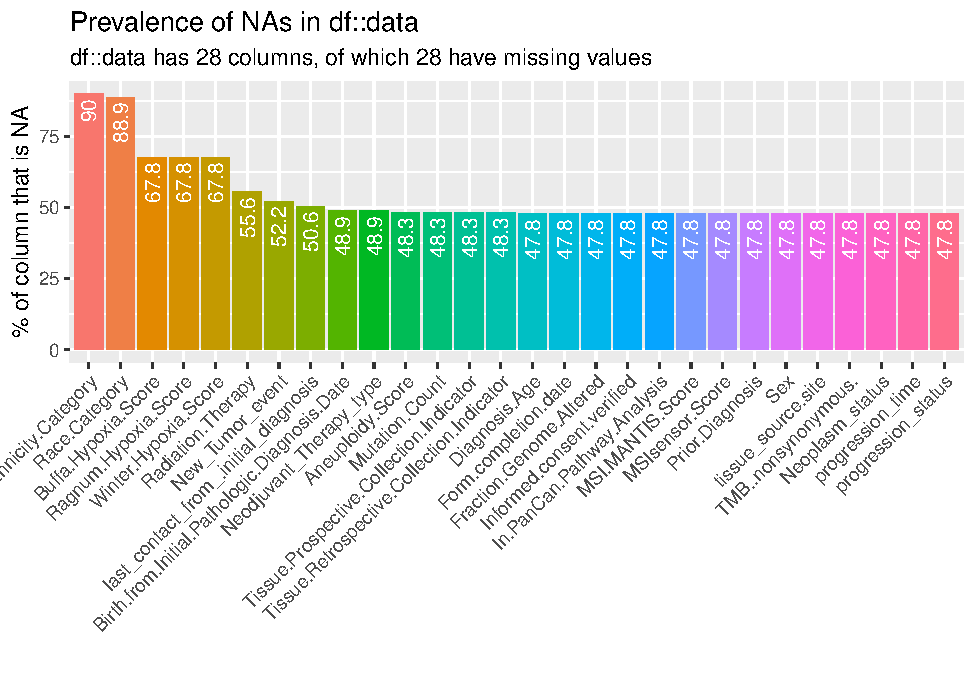
\includegraphics{Random_new_surv_4_files/figure-latex/unnamed-chunk-2-1.pdf}

\begin{Shaded}
\begin{Highlighting}[]
\NormalTok{missing }\OtherTok{=} \FunctionTok{inspect\_na}\NormalTok{(data)}
\NormalTok{missing[ , }\DecValTok{3}\NormalTok{] }\OtherTok{=} \FunctionTok{round}\NormalTok{(missing[ ,}\DecValTok{3}\NormalTok{], }\DecValTok{2}\NormalTok{)}
\FunctionTok{names}\NormalTok{(missing) }\OtherTok{=} \FunctionTok{c}\NormalTok{(}\StringTok{"variable"}\NormalTok{, }\StringTok{"count"}\NormalTok{, }\StringTok{"proportion"}\NormalTok{)}
\FunctionTok{require}\NormalTok{(kableExtra)}
\CommentTok{\# missing\textless{}{-}as.matrix.data.frame(missing)}
\FunctionTok{kable}\NormalTok{(missing)}
\end{Highlighting}
\end{Shaded}

\begin{tabular}{l|r|r}
\hline
variable & count & proportion\\
\hline
Ethnicity.Category & 162 & 90.00\\
\hline
Race.Category & 160 & 88.89\\
\hline
Buffa.Hypoxia.Score & 122 & 67.78\\
\hline
Ragnum.Hypoxia.Score & 122 & 67.78\\
\hline
Winter.Hypoxia.Score & 122 & 67.78\\
\hline
Radiation.Therapy & 100 & 55.56\\
\hline
New\_Tumor\_event & 94 & 52.22\\
\hline
last\_contact\_from\_.initial\_diagnosis & 91 & 50.56\\
\hline
Birth.from.Initial.Pathologic.Diagnosis.Date & 88 & 48.89\\
\hline
Neodjuvant\_Therapy\_type & 88 & 48.89\\
\hline
Aneuploidy.Score & 87 & 48.33\\
\hline
Mutation.Count & 87 & 48.33\\
\hline
Tissue.Prospective.Collection.Indicator & 87 & 48.33\\
\hline
Tissue.Retrospective.Collection.Indicator & 87 & 48.33\\
\hline
Diagnosis.Age & 86 & 47.78\\
\hline
Form.completion.date & 86 & 47.78\\
\hline
Fraction.Genome.Altered & 86 & 47.78\\
\hline
Informed.consent.verified & 86 & 47.78\\
\hline
In.PanCan.Pathway.Analysis & 86 & 47.78\\
\hline
MSI.MANTIS.Score & 86 & 47.78\\
\hline
MSIsensor.Score & 86 & 47.78\\
\hline
Prior.Diagnosis & 86 & 47.78\\
\hline
Sex & 86 & 47.78\\
\hline
tissue\_source.site & 86 & 47.78\\
\hline
TMB..nonsynonymous. & 86 & 47.78\\
\hline
Neoplasm\_status & 86 & 47.78\\
\hline
progression\_time & 86 & 47.78\\
\hline
progression\_status & 86 & 47.78\\
\hline
\end{tabular}

\begin{Shaded}
\begin{Highlighting}[]
\CommentTok{\# as.data.frame.matrix(missing)}
\CommentTok{\# kable(as.da(missing))}
\end{Highlighting}
\end{Shaded}

\subsubsection{Rename long variables}

\begin{Shaded}
\begin{Highlighting}[]
\StringTok{"TMB{-}H means that the tumor has a high number of mutations. Doctors have found that}
\StringTok{certain immunotherapy drugs are more likely to work}
\StringTok{against TMB{-}H cancers. This is because the immune}
\StringTok{system may be able to find and attack cancer cells with high}
\StringTok{TMB more easily."}
\end{Highlighting}
\end{Shaded}

\begin{verbatim}
## [1] "TMB-H means that the tumor has a high number of mutations. Doctors have found that\ncertain immunotherapy drugs are more likely to work\nagainst TMB-H cancers. This is because the immune\nsystem may be able to find and attack cancer cells with high\nTMB more easily."
\end{verbatim}

\begin{Shaded}
\begin{Highlighting}[]
\StringTok{"Person neoplasm status...... You are correct, IMO:  tumor free does not mean normal, but rather whether (or not) the tumor (neoplasm) continues to be present.  It is a statement about the progression (or not) of the original disease; whereas normal is a statement that there was no disease to begin with."}
\end{Highlighting}
\end{Shaded}

\begin{verbatim}
## [1] "Person neoplasm status...... You are correct, IMO:  tumor free does not mean normal, but rather whether (or not) the tumor (neoplasm) continues to be present.  It is a statement about the progression (or not) of the original disease; whereas normal is a statement that there was no disease to begin with."
\end{verbatim}

\newpage
\subsubsection{Re-coding variables}

\begin{Shaded}
\begin{Highlighting}[]
\CommentTok{\# newdata$Neodjuvant\_Therapy\_type \textless{}{-} factor(newdata$Neodjuvant\_Therapy\_type,}
\CommentTok{\#                                     levels=c("No","Yes"),}
\CommentTok{\#                                     labels=c("No","Yes")) all were "no"}


\NormalTok{data}\SpecialCharTok{$}\NormalTok{In.PanCan.Pathway.Analysis}\OtherTok{\textless{}{-}}\FunctionTok{factor}\NormalTok{(data}\SpecialCharTok{$}\NormalTok{In.PanCan.Pathway.Analysis,}
                                           \AttributeTok{levels=}\FunctionTok{c}\NormalTok{(}\StringTok{"No"}\NormalTok{,}\StringTok{"Yes"}\NormalTok{),}
                                           \AttributeTok{labels=}\FunctionTok{c}\NormalTok{(}\StringTok{"No"}\NormalTok{,}\StringTok{"Yes"}\NormalTok{))}


\NormalTok{data}\SpecialCharTok{$}\NormalTok{Prior.Diagnosis}\OtherTok{\textless{}{-}}\FunctionTok{factor}\NormalTok{(data}\SpecialCharTok{$}\NormalTok{Prior.Diagnosis, }
                                \AttributeTok{levels=}\FunctionTok{c}\NormalTok{(}\StringTok{"No"}\NormalTok{,}\StringTok{"Yes"}\NormalTok{),}
                                \AttributeTok{labels=}\FunctionTok{c}\NormalTok{(}\StringTok{"No"}\NormalTok{,}\StringTok{"Yes"}\NormalTok{))}
  

\NormalTok{data}\SpecialCharTok{$}\NormalTok{tissue\_source.site}\OtherTok{\textless{}{-}}\FunctionTok{factor}\NormalTok{(data}\SpecialCharTok{$}\NormalTok{tissue\_source.site,}
                                   \AttributeTok{levels =} \FunctionTok{c}\NormalTok{(}\StringTok{"university"}\NormalTok{,}\StringTok{"Biotech \& Pharma"}\NormalTok{,}\StringTok{"Hospital"}\NormalTok{,}\StringTok{"Research center"}\NormalTok{),}
                                                          \AttributeTok{labels=}\FunctionTok{c}\NormalTok{(}\StringTok{"university"}\NormalTok{,}\StringTok{"biotech\_pharma"}\NormalTok{,}\StringTok{"hospital"}\NormalTok{,}\StringTok{"research\_centers"}\NormalTok{))}


\NormalTok{data}\SpecialCharTok{$}\NormalTok{New\_Tumor\_event }\OtherTok{\textless{}{-}} \FunctionTok{factor}\NormalTok{(data}\SpecialCharTok{$}\NormalTok{New\_Tumor\_event,}
                                    \AttributeTok{levels=}\FunctionTok{c}\NormalTok{(}\StringTok{"No"}\NormalTok{,}\StringTok{"Yes"}\NormalTok{),}
                                    \AttributeTok{labels=}\FunctionTok{c}\NormalTok{(}\StringTok{"No"}\NormalTok{,}\StringTok{"Yes"}\NormalTok{))}


\NormalTok{data}\SpecialCharTok{$}\NormalTok{Radiation.Therapy }\OtherTok{\textless{}{-}} \FunctionTok{factor}\NormalTok{(data}\SpecialCharTok{$}\NormalTok{Radiation.Therapy,}
                                    \AttributeTok{levels=}\FunctionTok{c}\NormalTok{(}\StringTok{"No"}\NormalTok{,}\StringTok{"Yes"}\NormalTok{),}
                                    \AttributeTok{labels=}\FunctionTok{c}\NormalTok{(}\StringTok{"No"}\NormalTok{,}\StringTok{"Yes"}\NormalTok{))}

\CommentTok{\#all white , no adjuvant therapy}
\FunctionTok{str}\NormalTok{(data)}
\end{Highlighting}
\end{Shaded}

\begin{verbatim}
## 'data.frame':    180 obs. of  28 variables:
##  $ Diagnosis.Age                               : int  NA 64 65 48 NA 57 65 66 57 67 ...
##  $ Aneuploidy.Score                            : int  NA 0 3 0 NA 0 2 1 0 5 ...
##  $ Buffa.Hypoxia.Score                         : int  NA -31 -17 -13 NA -37 -29 -33 -31 -29 ...
##  $ last_contact_from_.initial_diagnosis        : int  NA 31 62 62 NA 91 1427 2118 1882 1115 ...
##  $ Birth.from.Initial.Pathologic.Diagnosis.Date: int  NA -23649 -23803 -17807 NA -21002 -24072 -24313 -20854 -24535 ...
##  $ Ethnicity.Category                          : chr  NA "Not Hispanic Or Latino" "Not Hispanic Or Latino" "Not Hispanic Or Latino" ...
##  $ Form.completion.date                        : chr  NA "3/21/2012" "3/21/2012" "3/16/2012" ...
##  $ Fraction.Genome.Altered                     : num  NA 0.0125 0.2071 0.0284 NA ...
##  $ Neodjuvant_Therapy_type                     : chr  NA "No" "No" "No" ...
##  $ Informed.consent.verified                   : chr  NA "Yes" "Yes" "Yes" ...
##  $ In.PanCan.Pathway.Analysis                  : Factor w/ 2 levels "No","Yes": NA 2 2 2 NA 2 2 2 2 2 ...
##  $ MSI.MANTIS.Score                            : num  NA 0.266 0.272 0.34 NA ...
##  $ MSIsensor.Score                             : num  NA 0 0.01 0.2 NA 0 0.01 0 0 0.31 ...
##  $ Mutation.Count                              : int  NA 33 78 108 NA 34 40 31 37 59 ...
##  $ New_Tumor_event                             : Factor w/ 2 levels "No","Yes": NA NA NA NA NA NA 1 2 1 2 ...
##  $ Prior.Diagnosis                             : Factor w/ 2 levels "No","Yes": NA 1 1 1 NA 1 1 1 1 1 ...
##  $ Race.Category                               : chr  NA "white" "white" "white" ...
##  $ Radiation.Therapy                           : Factor w/ 2 levels "No","Yes": NA NA NA NA NA NA 1 1 1 1 ...
##  $ Ragnum.Hypoxia.Score                        : int  NA -20 -2 6 NA -20 -20 -20 -12 -8 ...
##  $ Sex                                         : chr  NA "Male" "Male" "Male" ...
##  $ Tissue.Prospective.Collection.Indicator     : chr  NA "Yes" "Yes" "Yes" ...
##  $ Tissue.Retrospective.Collection.Indicator   : chr  NA "No" "No" "No" ...
##  $ tissue_source.site                          : Factor w/ 4 levels "university","biotech_pharma",..: NA NA NA NA NA NA 1 1 1 1 ...
##  $ TMB..nonsynonymous.                         : num  NA 1.1 2.6 3.57 NA ...
##  $ Winter.Hypoxia.Score                        : int  NA -28 -16 -24 NA -40 -30 -26 -40 -32 ...
##  $ Neoplasm_status                             : chr  NA "with_tumor" "with_tumor" "with_tumor" ...
##  $ progression_time                            : num  NA 1.02 2.04 2.04 NA ...
##  $ progression_status                          : int  NA 1 1 1 NA 1 1 2 2 2 ...
\end{verbatim}

\newpage
\section{Generate Random subsets from entire data}

\begin{Shaded}
\begin{Highlighting}[]
\NormalTok{ndata}\OtherTok{\textless{}{-}}\NormalTok{data}
\FunctionTok{set.seed}\NormalTok{(}\DecValTok{1}\NormalTok{)}
\FunctionTok{library}\NormalTok{(dplyr)}
\CommentTok{\# Generate different random rows as subsets to be used for analysis  }
\NormalTok{ sample\_data1}\OtherTok{\textless{}{-}}\FunctionTok{sample\_n}\NormalTok{(ndata, }\DecValTok{100}\NormalTok{) }\CommentTok{\#100   }
\NormalTok{ sample\_data2}\OtherTok{\textless{}{-}}\FunctionTok{sample\_n}\NormalTok{(ndata, }\DecValTok{90}\NormalTok{) }\CommentTok{\#90}
\NormalTok{ sample\_data3}\OtherTok{\textless{}{-}}\FunctionTok{sample\_n}\NormalTok{(ndata, }\DecValTok{90}\NormalTok{) }\CommentTok{\#90}
\NormalTok{ sample\_data4}\OtherTok{\textless{}{-}}\FunctionTok{sample\_n}\NormalTok{(ndata, }\DecValTok{80}\NormalTok{) }\CommentTok{\#80}
\end{Highlighting}
\end{Shaded}

\newpage
\section{KM Curve - Survival probability with Radiation Therapy of 100 sampled subjects}

\begin{Shaded}
\begin{Highlighting}[]
\FunctionTok{library}\NormalTok{(}\StringTok{"survival"}\NormalTok{)}
\FunctionTok{library}\NormalTok{(}\StringTok{"survminer"}\NormalTok{)}

\NormalTok{fit2a}\OtherTok{\textless{}{-}}\FunctionTok{survfit}\NormalTok{(}\FunctionTok{Surv}\NormalTok{(sample\_data1}\SpecialCharTok{$}\NormalTok{progression\_time, sample\_data1}\SpecialCharTok{$}\NormalTok{progression\_status}\SpecialCharTok{==}\DecValTok{2}\NormalTok{)}\SpecialCharTok{\textasciitilde{}}
\NormalTok{                   sample\_data1}\SpecialCharTok{$}\NormalTok{Radiation.Therapy, }\AttributeTok{data=}\NormalTok{sample\_data1)}
\FunctionTok{print}\NormalTok{(fit2a)}
\end{Highlighting}
\end{Shaded}

\begin{verbatim}
## Call: survfit(formula = Surv(sample_data1$progression_time, sample_data1$progression_status == 
##     2) ~ sample_data1$Radiation.Therapy, data = sample_data1)
## 
##    53 observations deleted due to missingness 
##                                     n events median 0.95LCL 0.95UCL
## sample_data1$Radiation.Therapy=No  33     20   30.4    22.3      NA
## sample_data1$Radiation.Therapy=Yes 14      6   48.5    24.3      NA
\end{verbatim}

\begin{Shaded}
\begin{Highlighting}[]
\FunctionTok{summary}\NormalTok{(fit2a)}\SpecialCharTok{$}\NormalTok{table}
\end{Highlighting}
\end{Shaded}

\begin{verbatim}
##                                    records n.max n.start events    rmean
## sample_data1$Radiation.Therapy=No       33    33      33     20 47.76400
## sample_data1$Radiation.Therapy=Yes      14    14      14      6 32.67909
##                                    se(rmean)   median  0.95LCL 0.95UCL
## sample_data1$Radiation.Therapy=No  10.165516 30.41063 22.32304      NA
## sample_data1$Radiation.Therapy=Yes  5.631744 48.52550 24.32850      NA
\end{verbatim}

\begin{Shaded}
\begin{Highlighting}[]
\FunctionTok{ggsurvplot}\NormalTok{(fit2a,}
          \CommentTok{\#legend.labs=c("tumor\_free", "with\_tumor"),}
          \AttributeTok{pval =} \ConstantTok{TRUE}\NormalTok{, }\AttributeTok{conf.int =}\NormalTok{ F,}
          \AttributeTok{risk.table =} \ConstantTok{TRUE}\NormalTok{, }\CommentTok{\# Add risk table}
          \AttributeTok{risk.table.col =} \StringTok{"strata"}\NormalTok{, }\CommentTok{\# Change risk table color by groups}
          \AttributeTok{linetype =} \StringTok{"strata"}\NormalTok{, }\CommentTok{\# Change line type by groups}
          \AttributeTok{surv.median.line =} \StringTok{"hv"}\NormalTok{, }\CommentTok{\# Specify median survival}
          \AttributeTok{ggtheme =} \FunctionTok{theme\_bw}\NormalTok{(), }\CommentTok{\# Change ggplot2 theme}
          \AttributeTok{palette =} \FunctionTok{c}\NormalTok{(}\StringTok{"\#E7B800"}\NormalTok{, }\StringTok{"\#2E9FDF"}\NormalTok{))}
\end{Highlighting}
\end{Shaded}

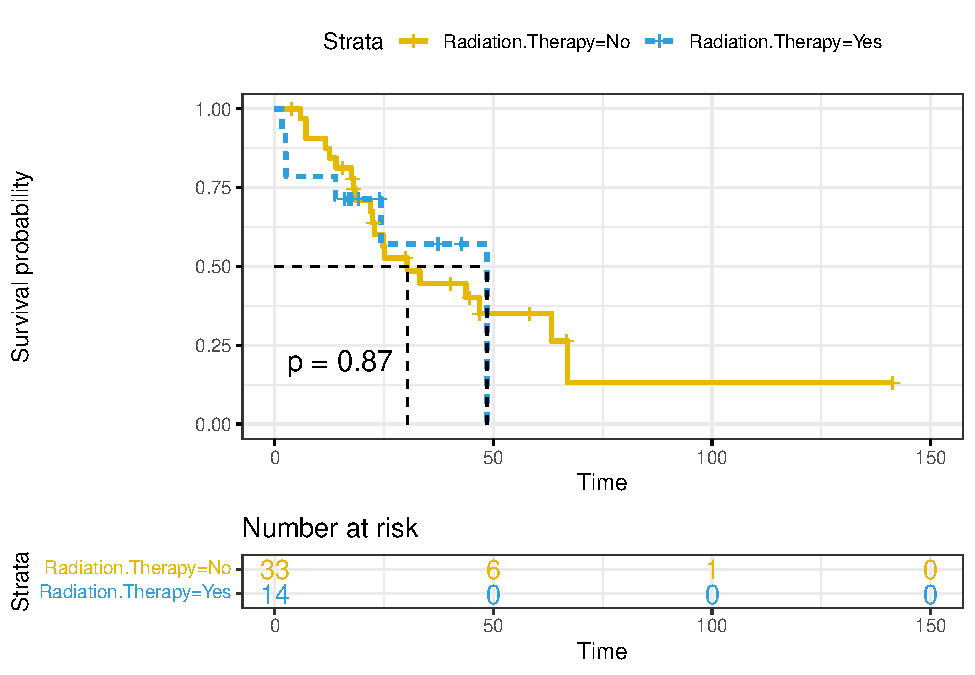
\includegraphics{Random_new_surv_4_files/figure-latex/unnamed-chunk-7-1.pdf}

\begin{Shaded}
\begin{Highlighting}[]
\CommentTok{\#1 {-} censored \& 2{-} progression}
\CommentTok{\#1 {-} tumor\_free \& 2 with tumor .....neoplasm status }
\CommentTok{\#1 {-} NO \& 2{-}YES .....TREATMENT CODE}
\end{Highlighting}
\end{Shaded}

\newpage
\section{KM Curve - Survival probability with Radiation Therapy of 90 sampled subjects}

\begin{Shaded}
\begin{Highlighting}[]
\NormalTok{fit2b }\OtherTok{\textless{}{-}} \FunctionTok{survfit}\NormalTok{(}\FunctionTok{Surv}\NormalTok{(sample\_data2}\SpecialCharTok{$}\NormalTok{progression\_time,sample\_data2}\SpecialCharTok{$}\NormalTok{progression\_status}\SpecialCharTok{==}\DecValTok{2}\NormalTok{) }\SpecialCharTok{\textasciitilde{}}
\NormalTok{                   sample\_data2}\SpecialCharTok{$}\NormalTok{Radiation.Therapy, }\AttributeTok{data=}\NormalTok{sample\_data2)}
\FunctionTok{print}\NormalTok{(fit2b)}
\end{Highlighting}
\end{Shaded}

\begin{verbatim}
## Call: survfit(formula = Surv(sample_data2$progression_time, sample_data2$progression_status == 
##     2) ~ sample_data2$Radiation.Therapy, data = sample_data2)
## 
##    48 observations deleted due to missingness 
##                                     n events median 0.95LCL 0.95UCL
## sample_data2$Radiation.Therapy=No  31     22   22.8    14.5    43.7
## sample_data2$Radiation.Therapy=Yes 11      5   48.5    24.3      NA
\end{verbatim}

\begin{Shaded}
\begin{Highlighting}[]
\FunctionTok{summary}\NormalTok{(fit2b)}\SpecialCharTok{$}\NormalTok{table}
\end{Highlighting}
\end{Shaded}

\begin{verbatim}
##                                    records n.max n.start events    rmean
## sample_data2$Radiation.Therapy=No       31    31      31     22 28.95121
## sample_data2$Radiation.Therapy=Yes      11    11      11      5 33.41254
##                                    se(rmean)   median  0.95LCL  0.95UCL
## sample_data2$Radiation.Therapy=No   4.046563 22.75044 14.53135 43.69267
## sample_data2$Radiation.Therapy=Yes  6.022552 48.52550 24.32850       NA
\end{verbatim}

\begin{Shaded}
\begin{Highlighting}[]
\FunctionTok{ggsurvplot}\NormalTok{(fit2b,}
          \CommentTok{\#legend.labs=c("tumor\_free", "with\_tumor"),}
          \AttributeTok{pval =} \ConstantTok{TRUE}\NormalTok{, }\AttributeTok{conf.int =}\NormalTok{ F,}
          \AttributeTok{risk.table =} \ConstantTok{TRUE}\NormalTok{, }\CommentTok{\# Add risk table}
          \AttributeTok{risk.table.col =} \StringTok{"strata"}\NormalTok{, }\CommentTok{\# Change risk table color by groups}
          \AttributeTok{linetype =} \StringTok{"strata"}\NormalTok{, }\CommentTok{\# Change line type by groups}
          \AttributeTok{surv.median.line =} \StringTok{"hv"}\NormalTok{, }\CommentTok{\# Specify median survival}
          \AttributeTok{ggtheme =} \FunctionTok{theme\_bw}\NormalTok{(), }\CommentTok{\# Change ggplot2 theme}
          \AttributeTok{palette =} \FunctionTok{c}\NormalTok{(}\StringTok{"\#E7B800"}\NormalTok{, }\StringTok{"\#2E9FDF"}\NormalTok{))}
\end{Highlighting}
\end{Shaded}

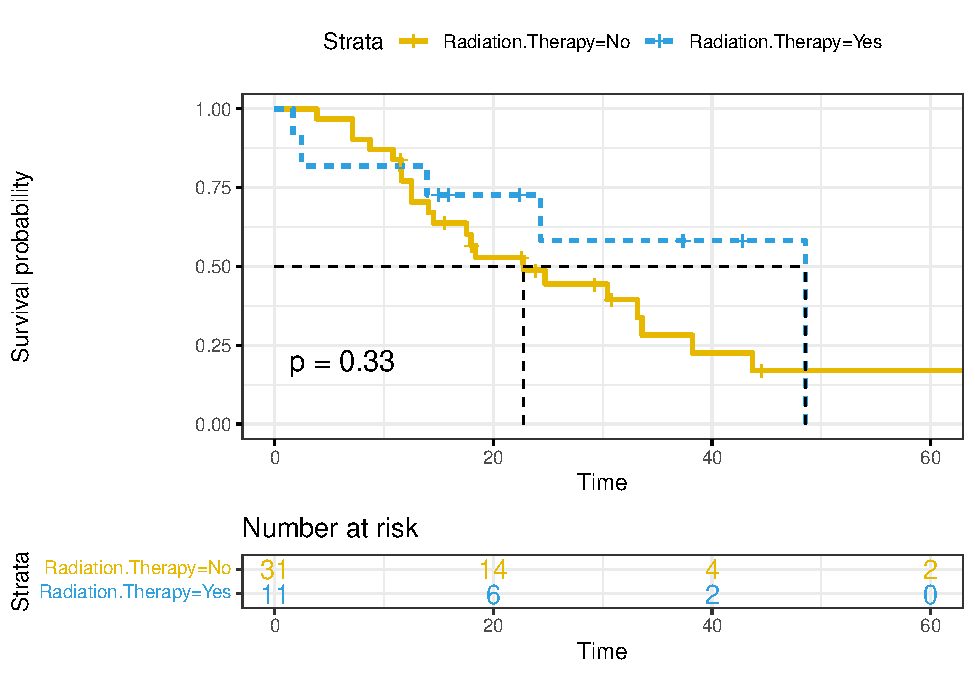
\includegraphics{Random_new_surv_4_files/figure-latex/unnamed-chunk-9-1.pdf}

\begin{Shaded}
\begin{Highlighting}[]
\CommentTok{\#1 {-} censored \& 2{-} progression}
\CommentTok{\#1 {-} tumor\_free \& 2 with tumor .....neoplasm status }
\CommentTok{\#1 {-} NO \& 2{-}YES .....TREATMENT CODE}
\end{Highlighting}
\end{Shaded}

\newpage
\section{KM Curve - Survival probability with Radiation Therapy of 90 sampled subjects}

\begin{Shaded}
\begin{Highlighting}[]
\NormalTok{fit2c }\OtherTok{\textless{}{-}} \FunctionTok{survfit}\NormalTok{(}\FunctionTok{Surv}\NormalTok{(sample\_data3}\SpecialCharTok{$}\NormalTok{progression\_time,sample\_data3}\SpecialCharTok{$}\NormalTok{progression\_status}\SpecialCharTok{==}\DecValTok{2}\NormalTok{) }\SpecialCharTok{\textasciitilde{}}
\NormalTok{                   sample\_data3}\SpecialCharTok{$}\NormalTok{Radiation.Therapy, }\AttributeTok{data=}\NormalTok{sample\_data3)}
\FunctionTok{print}\NormalTok{(fit2c)}
\end{Highlighting}
\end{Shaded}

\begin{verbatim}
## Call: survfit(formula = Surv(sample_data3$progression_time, sample_data3$progression_status == 
##     2) ~ sample_data3$Radiation.Therapy, data = sample_data3)
## 
##    55 observations deleted due to missingness 
##                                     n events median 0.95LCL 0.95UCL
## sample_data3$Radiation.Therapy=No  23     14   33.2    20.6      NA
## sample_data3$Radiation.Therapy=Yes 12      3     NA      NA      NA
\end{verbatim}

\begin{Shaded}
\begin{Highlighting}[]
\FunctionTok{summary}\NormalTok{(fit2c)}\SpecialCharTok{$}\NormalTok{table}
\end{Highlighting}
\end{Shaded}

\begin{verbatim}
##                                    records n.max n.start events    rmean
## sample_data3$Radiation.Therapy=No       23    23      23     14 34.92506
## sample_data3$Radiation.Therapy=Yes      12    12      12      3 51.50902
##                                    se(rmean)   median 0.95LCL 0.95UCL
## sample_data3$Radiation.Therapy=No   4.847872 33.17224 20.5806      NA
## sample_data3$Radiation.Therapy=Yes  7.624896       NA      NA      NA
\end{verbatim}

\begin{Shaded}
\begin{Highlighting}[]
\FunctionTok{ggsurvplot}\NormalTok{(fit2c,}
          \CommentTok{\#legend.labs=c("tumor\_free", "with\_tumor"),}
          \AttributeTok{pval =} \ConstantTok{TRUE}\NormalTok{, }\AttributeTok{conf.int =}\NormalTok{ F,}
          \AttributeTok{risk.table =} \ConstantTok{TRUE}\NormalTok{, }\CommentTok{\# Add risk table}
          \AttributeTok{risk.table.col =} \StringTok{"strata"}\NormalTok{, }\CommentTok{\# Change risk table color by groups}
          \AttributeTok{linetype =} \StringTok{"strata"}\NormalTok{, }\CommentTok{\# Change line type by groups}
          \AttributeTok{surv.median.line =} \StringTok{"hv"}\NormalTok{, }\CommentTok{\# Specify median survival}
          \AttributeTok{ggtheme =} \FunctionTok{theme\_bw}\NormalTok{(), }\CommentTok{\# Change ggplot2 theme}
          \AttributeTok{palette =} \FunctionTok{c}\NormalTok{(}\StringTok{"\#E7B800"}\NormalTok{, }\StringTok{"\#2E9FDF"}\NormalTok{))}
\end{Highlighting}
\end{Shaded}

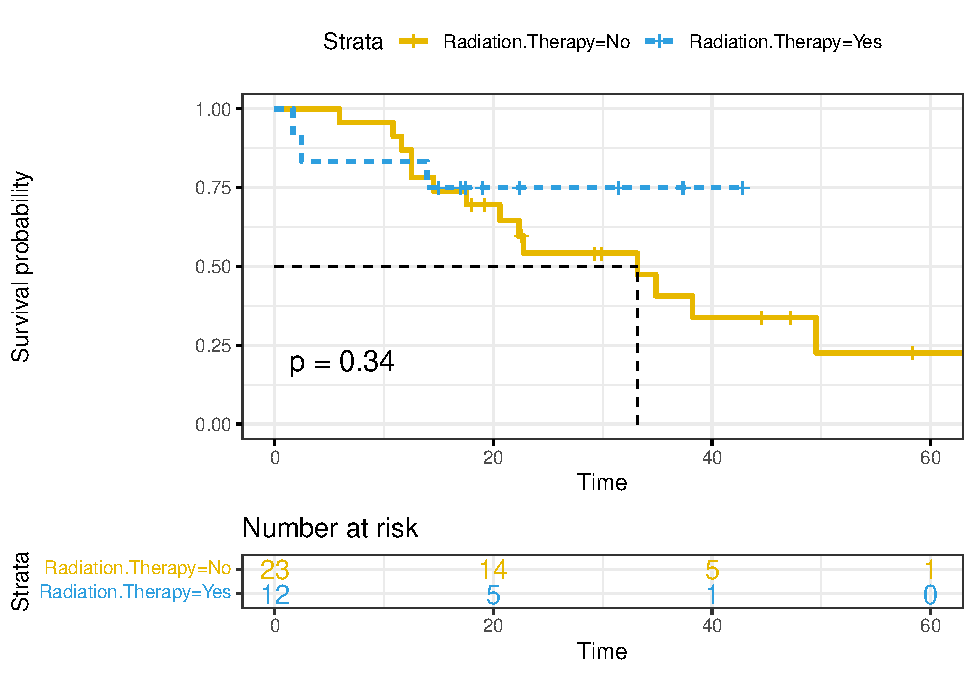
\includegraphics{Random_new_surv_4_files/figure-latex/unnamed-chunk-11-1.pdf}

\begin{Shaded}
\begin{Highlighting}[]
\CommentTok{\#1 {-} censored \& 2{-} progression}
\CommentTok{\#1 {-} tumor\_free \& 2 with tumor .....neoplasm status }
\CommentTok{\#1 {-} NO \& 2{-}YES .....TREATMENT CODE}
\end{Highlighting}
\end{Shaded}

\newpage
\section{KM Curve - Survival probability with Radiation Therapy of 80 sampled subjects}

\begin{Shaded}
\begin{Highlighting}[]
\NormalTok{fit2d }\OtherTok{\textless{}{-}} \FunctionTok{survfit}\NormalTok{(}\FunctionTok{Surv}\NormalTok{(sample\_data4}\SpecialCharTok{$}\NormalTok{progression\_time,sample\_data4}\SpecialCharTok{$}\NormalTok{progression\_status}\SpecialCharTok{==}\DecValTok{2}\NormalTok{) }\SpecialCharTok{\textasciitilde{}}
\NormalTok{                   sample\_data4}\SpecialCharTok{$}\NormalTok{Radiation.Therapy, }\AttributeTok{data=}\NormalTok{sample\_data4)}
\FunctionTok{print}\NormalTok{(fit2d)}
\end{Highlighting}
\end{Shaded}

\begin{verbatim}
## Call: survfit(formula = Surv(sample_data4$progression_time, sample_data4$progression_status == 
##     2) ~ sample_data4$Radiation.Therapy, data = sample_data4)
## 
##    49 observations deleted due to missingness 
##                                     n events median 0.95LCL 0.95UCL
## sample_data4$Radiation.Therapy=No  22     14   33.2    21.8      NA
## sample_data4$Radiation.Therapy=Yes  9      3   45.2    24.3      NA
\end{verbatim}

\begin{Shaded}
\begin{Highlighting}[]
\FunctionTok{summary}\NormalTok{(fit2d)}\SpecialCharTok{$}\NormalTok{table}
\end{Highlighting}
\end{Shaded}

\begin{verbatim}
##                                    records n.max n.start events    rmean
## sample_data4$Radiation.Therapy=No       22    22      22     14 43.65753
## sample_data4$Radiation.Therapy=Yes       9     9       9      3 35.85349
##                                    se(rmean)   median 0.95LCL 0.95UCL
## sample_data4$Radiation.Therapy=No  10.806475 33.17224 21.8299      NA
## sample_data4$Radiation.Therapy=Yes  5.617246 45.23786 24.3285      NA
\end{verbatim}

\begin{Shaded}
\begin{Highlighting}[]
\FunctionTok{ggsurvplot}\NormalTok{(fit2d,}
          \CommentTok{\#legend.labs=c("tumor\_free", "with\_tumor"),}
          \AttributeTok{pval =} \ConstantTok{TRUE}\NormalTok{, }\AttributeTok{conf.int =}\NormalTok{ F,}
          \AttributeTok{risk.table =} \ConstantTok{TRUE}\NormalTok{, }\CommentTok{\# Add risk table}
          \AttributeTok{risk.table.col =} \StringTok{"strata"}\NormalTok{, }\CommentTok{\# Change risk table color by groups}
          \AttributeTok{linetype =} \StringTok{"strata"}\NormalTok{, }\CommentTok{\# Change line type by groups}
          \AttributeTok{surv.median.line =} \StringTok{"hv"}\NormalTok{, }\CommentTok{\# Specify median survival}
          \AttributeTok{ggtheme =} \FunctionTok{theme\_bw}\NormalTok{(), }\CommentTok{\# Change ggplot2 theme}
          \AttributeTok{palette =} \FunctionTok{c}\NormalTok{(}\StringTok{"\#E7B800"}\NormalTok{, }\StringTok{"\#2E9FDF"}\NormalTok{))}
\end{Highlighting}
\end{Shaded}

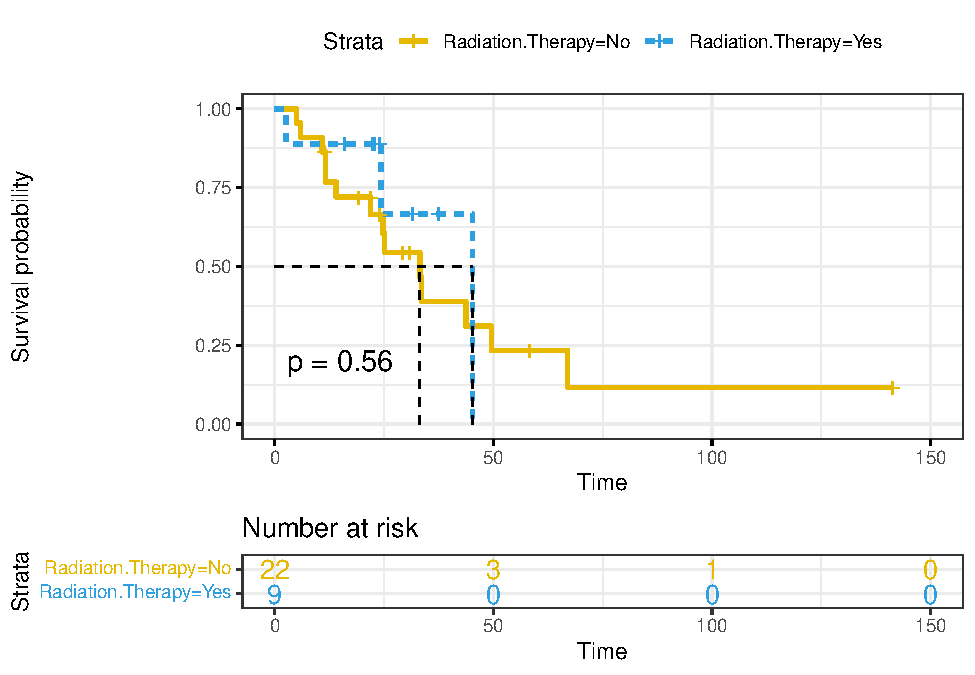
\includegraphics{Random_new_surv_4_files/figure-latex/unnamed-chunk-13-1.pdf}

\begin{Shaded}
\begin{Highlighting}[]
\CommentTok{\#1 {-} censored \& 2{-} progression}
\end{Highlighting}
\end{Shaded}


\end{document}
